 \section{Durchführung}
\label{sec:Durchführung}

\subsection{Aufbau}

Für die Spektralmessungen wird ein Gitterspektralapparat \ref{fig:Gspa}
verwendet. An das eine Ende wird jeweils die Lampe gestellt, sodass das Licht
in die Spaltblende 1.1 fällt. Diese kann mit der Dort angebrachten Schraube
verstellt werden, sodass die Spaltbilder schärfer werden. Das Licht bewegt sich
durch ein Gitter 2 und wird dann gebeugt.
Der zweite Teil des Apparats ist ein schwenkbares Fernrohr 3, mit
welchem das Spektrum beobachtet werden kann. Dort sind eine Objektiv- und
Okularlinse mit Fadenkreuz eingebaut, sodass mit einem Okularmikrometer bei 3.2
feinverstellt werden kann. Dafür sollte das Fernrohr allerdings zuerst mit der
Rändelschraube 3.1 arretiert werden. An der Teilkreisplatte 4 in der
Mitte kann der Winkel abgelesen werden.

\begin{figure}
  \centering
  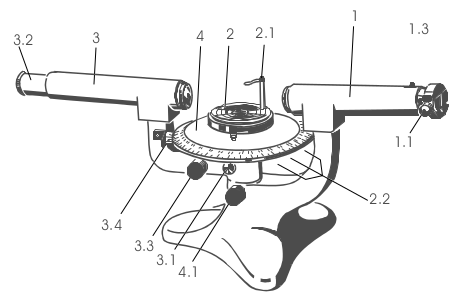
\includegraphics[height=5cm]{MeinFotoalbum:)/Apparatur.png}
  \caption{Aufbau der Apparatur. Die Lampe wird vor das rechte Ende gestellt.
  \cite{anleitung}}
  \label{fig:Gspa}
\end{figure}

\subsection{Messprogramm}

\subsubsection{Spektrallinien des He-Spektrums}

\begin{enumerate}

  \item Nachdem die Helium-Lampe vor die Apparatur gestellt wird, wird der
  Winkel am Nullten Maximum ausgemessen.

  \item Als nächstes werden die wichtigsten sichtbaren Spektrallinien
  von Helium aus Tabelle \ref{tab:helium} ausgemessen. Es werden insgesamt
  neun Messwerte notiert.

\end{enumerate}

\begin{table}
  \centering
  \begin{tabular}{S S S}
    \toprule
    {$\lambda/\si{\nano\meter}$} & {Farbe} & {Intensität} \\
    \midrule
    706.5 & \text{dunkelrot} & \text{schwach} \\
    667.8 & \text{rot} & \text{stark} \\
    587.6 & \text{gelb} & \text{stark} \\
    504.8 & \text{grün} & \text{schwach} \\
    501.6 & \text{grün} & \text{stark} \\
    492.2 & \text{blaugrün} & \text{mittel} \\
    471.3 & \text{blau} & \text{stark} \\
    447.1 & \text{violett} & \text{stark} \\
    438.8 & \text{violett} & \text{schwach} \\
    \bottomrule
  \end{tabular}
  \caption{Die wichtigsten sichtbaren Spektrallinien von Helium.\cite{anleitung}}
  \label{tab:helium}
\end{table}

\subsubsection{Dublettlinien verschiedener Elemente}

\begin{enumerate}

  \item Vor jeder der folgenden Messungen wird erneut der Nullwinkel bestimmt.

  \item Es sollen die Beugungswinkel der in Tabelle \ref{tab:beug} aufgezählten
  Dublettlinien gemessen werden. Liegen die beiden Linien eines Dubletts nah
  genug aneinander, darf der Wert gemittelt werden. Ansonsten sollten pro
  Dublett zwei Messwerte aufgenommen werden. Es sollten also mindestens
  acht Werte notiert werden.

\end{enumerate}

Bei Tabelle \ref{tab:beug} ist zu beachten, dass das gesuchte Dublett bei
Rubidium aus der dritten und vierten roten Linie besteht.
Die Lage der Dublettlinien bei Kalium sind in Abbildung \ref{fig:kalium}
skizziert.

\begin{figure}
  \centering
  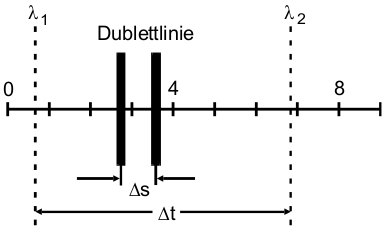
\includegraphics[height=3.5cm]{MeinFotoalbum:)/Dubletts.png}
  \caption{Lage der vier grünen sowie der vier gelben Linien. \cite{anleitung}}
  \label{fig:kalium}
\end{figure}

\begin{table}
  \centering
  \begin{tabular}{S S}
    \toprule
    {Element und Farbe} & {Anzahl Dubletts} \\
    \midrule
    \text{Na, rot} & 1 \\
    \text{Na, gelb} & 1 \\
    \text{Na, grüngelb} & 1 \\
    \text{Ka, gelb} & 2 \\
    \text{Ka, grün} & 2 \\
    \text{Rb, rot} & 1 \\
    \bottomrule
  \end{tabular}
  \caption{Dublettlinien, die in diesem Versuch gemessen werden sollen.}
  \label{tab:beug}
\end{table}

\subsubsection{Distanzen der Dubletts}

\begin{enumerate}

  \item Vor den folgenden Messungen sollte das Gerät jeweils mit der
  Rändelschraube arretiert werden.

  \item Zunächst wird der in Kapitel \ref{sec:AvD} erwähnte Abstand
  $\increment t$ zwischen zwei bekannten Linien eines Dubletts mit
  Hilfe des Okularmikrometers bestimmt.

  \item Nun sollen die Dublettlinien aus Tabelle \ref{tab:beug} ausgemessen
  werden. Es werden also insgesamt 16 Messwerte und damit 8 Differenzen
  notiert

\end{enumerate}
